\chapter{Future Work}

SweetPea is a work-in-progress. The ultimate vision for SweetPea is for it to be a convenient system for describing diverse types of experimental designs, and then quickly and seamlessly integrating the resulting experimental sequences with the users' existing experiment running pipelines. Ideally, SweetPea could be a tool in dialog with the user; the user should be able to use SweetPea to iteratively explore the space of possible satisfiable experimental designs. To achieve this vision, SweetPea will need more high-level language features, and more runtime support for debugging unsatisfiable experiments. It would also benefit by an expansion of its existing features such as built-in support for discretizing continuous functions for use as levels, weighted crossings and support for arbitrary DerivationFunctions.

Another possible future direction for SweetPea which is orthogonal to this vision is to expand SweetPea to support experiments in other domains beyond psychology, which may involve other experimental structures. Possible candidates for fields that could benefit from an experimental design description language are biology and machine learning; in both biology and machine learning, however, the the notion of a trial may require broadening and/or redefinition, and may lack a notion of ordering. This means that SweetPea would likely need to support more semantics for describing subsets of the crossing space, and applying constraints to these subsets.

%%% ~~~~~~~~~~~~~~~~~~~~~~~~~~~~~~~~~~~~~~~~~~~~~~~~~~~~~~~~~~~~~~~~~~~~~~~~~~~
\section{Language Wishlist}

This section describes some language features which would facilitate supporting a wider range of experiments.

\subsection{Windows on Counting Constraints}
Currently, counting constraints are specified using the \texttt{AtMostKInARow}, \texttt{ExactlyKInARow} or \texttt{AtLeastKInARow} constructors. These operate over the entire experimental sequence, which limits the constraints they can express. If these constraints were expanded to operate over a window, in the way that derived levels do, they could be used to express a wider range of desired constraints, including more complicated balancing constraints.

\subsection{General Case Derivations}

Currently, SweetPea can handle transition and congruency constraints. These are common constraints in task switching experiments, but to be able to represent a wider variety of experiments, SweetPea needs to handle arbitrary derivation functions. Recall that a derivation function is a Python function with the function signature:

\begin{verbatim}
  DerivationFunction = ( Listof( FactorName )... ) -> Boolean
\end{verbatim}

Derivation functions are used by windows, along with a list of factors to which this function should be symbolically applied:

\begin{verbatim}
  Window = Stride Width DerivationFunction Listof( FactorName )
\end{verbatim}

To encode any function which takes some number of lists of factor names, and evaluates the truth value of those factors, we could use a truth table encoding. This means that we could generate a truth table which represented every possible combination of the input variables and compute what the output value of the derivation function would be for every input combination. We could then allocate a new level by specifying that that level is true iff (all the rows of the truth table which are true). We could then further simplify this truth table by the Quine-Mccluskey algorithm. This approach would be limited by the number of variables in the truth table, and another approach may be necessary to support designs which express conditions that depend on the state of many boolean variables.

% \subsection{Syntactic Sugar}
% One of the examples we saw in Chapter 3 was:
% \begin{verbatim}
% ink_color = ("ink_color", ["red", "blue"])
% text      = ("text",      ["red", "blue"])
%
% def congruent(ink_colors, texts):
%   if ink_colors[0] == texts[0]:
%     return True
%   return False
%
% def incongruent(ink_colors, texts):
%   return not congruent(ink_colors, texts)
%
% con_level  = DerivedLevel("con",
%                WithinTrial(congruent, [ink_color, text]))
% inc_level  = DerivedLevel("inc",
%                WithinTrial(incongruent, [ink_color, text])
% congruenceFactor = Factor("congruent?", [con_level, inc_level])
% \end{verbatim}
% It is common that

\subsection{Weighted Crossings}
It would be useful to have a mechanism to specify a way to over- or under-sample a full crossing. A use-case for this is a version of the Stroop experiment with 3 colors; in a full crossing there are 3 congruent stimuli, and 6 incongruent stimuli. It is well-motivated to want to balance the number of congruent and incongruent stimuli. One can imagine either undersampling the incongruent stimuli (choosing 3 of the 6 with uniform likelihood), or over-sampling the congruent stimuli (such that each congruent stimuli occurs twice). More generally, it will be worth investigating more ways of specifying parts of the space of the full crossing, including regularized approaches (such as Latin Square designs).


\subsection{Sampling Continuous Factors}
Some experiments may contain levels which represent continuous values, such as sampling colors from the continuous color spectrum. We can currently represent these experiments by binning the continuous values into a number of discrete levels-- but can we do better? This is challenging because the translation to SAT is necessarily discrete. Perhaps this could be supported as a pre- and postprocessing step, or perhaps Unigen could natively support this. The user could specify the continuous value, and SweetPea could perform binning, find a solution and add random noise to the solution to simulate sampling from a continuous distribution.

\subsection{Automated Experimental Design}
In the spirit of declarative programming, it would be valuable to extend SweetPea to automatically derive the minimal set of counterbalancing conditions that satisfy the specified statistical analysis. Specifically, we may wish to provide an interface for the ANOVA (ANalysis Of VAriance) technique, which would allow researchers to state "contrast red with blue" instead of explicitly stating a design that does so. This higher-level interface will make it easier to specify experiments that accurately match the desired statistical analysis. Perhaps such an interface would also support iterative and interactive experiment specification. For instance, if multiple experiments match a desired statistical analysis, perhaps the user can use SweetPea to explore the options and trade-offs of each of those possible experiments.

%\subsection{Syntactic Sugar}
%- don't have to write the name of the factor when the level name is unique


%%% ~~~~~~~~~~~~~~~~~~~~~~~~~~~~~~~~~~~~~~~~~~~~~~~~~~~~~~~~~~~~~~~~~~~~~~~~~~~
\section{Runtime Wishlist}

This section describes some runtime features which would facilitate a more interactive and usable environment.


\subsection{Verified Core}

SweetPea promises to make it easier to write correct experiments; this promise can only be true if SweetPea itself doesn't contain bugs. The boolean encoding parts of the code, especially the counting constraint encoding, is ripe for bugs because it produces a CNF formula, which is difficult for humans to read and verify. Currently, we protect against bugs through exhaustive testing. In the future, it would be better to formally verify that these transformations are correct.

\subsection{Debugging unSAT Experiments}

If a user writes down an experimental design which is overspecified, the SAT-sampler will state that the constraints are unsatisfiable. This is not as helpful as it could be-- why is it overspecified? Developing debugging support would create a more pleasant user experience. One possible approach is that some SAT-solvers can provide a \emph{minimally unsatisifiable core}, which specifies what set of variables lead to a contradicting assignment. It may be possible to use this minimally unsatisfiable core to translate back to which constraints over which the levels are reported to be contradictory.

\subsection{Iterative Experimental Design and Partial Satisfiability}

Extending the idea of adding support for debugging unsatisfiable experiments, it would be great to have SweetPea be a tool for exploring the edge of satisfiability. For instance, perhaps a researcher could attempt to specify an ambitious experimental design which tests multiple things at once: perhaps in the future, SweetPea could allow them to iteratively explore which subsets of their overconstrained design are satisfiable. One technique for facilitating this is some SAT solvers allow you to push / pop individual clauses; perhaps this fine-grain precision can be used to find the most constraints which can be simultaneously satisfied.

% \subsection{Optimizations}
%
% Finally, there are some optimizations in that could be applied to the encodings discussed in Chapters 3, 4 and 5. A few examples are:
%
% Unigen supports "xor" constraints, in addition to the usual CNF formula. This is useful because adders are based on an "xor" operation internally. The current implementation desugars these xors into CNF, but perhaps explicitly specifying these xors might make the search simpler for the sampler, resulting in faster runtimes.
%
% The truth tables currently used to represent derivation functions can be compressed / optimized using the Quine-McCluskey algorithm. Further
%
% - choice of SAT encodings and variable v. clauses

%
% \begin{figure}
%     \centerline{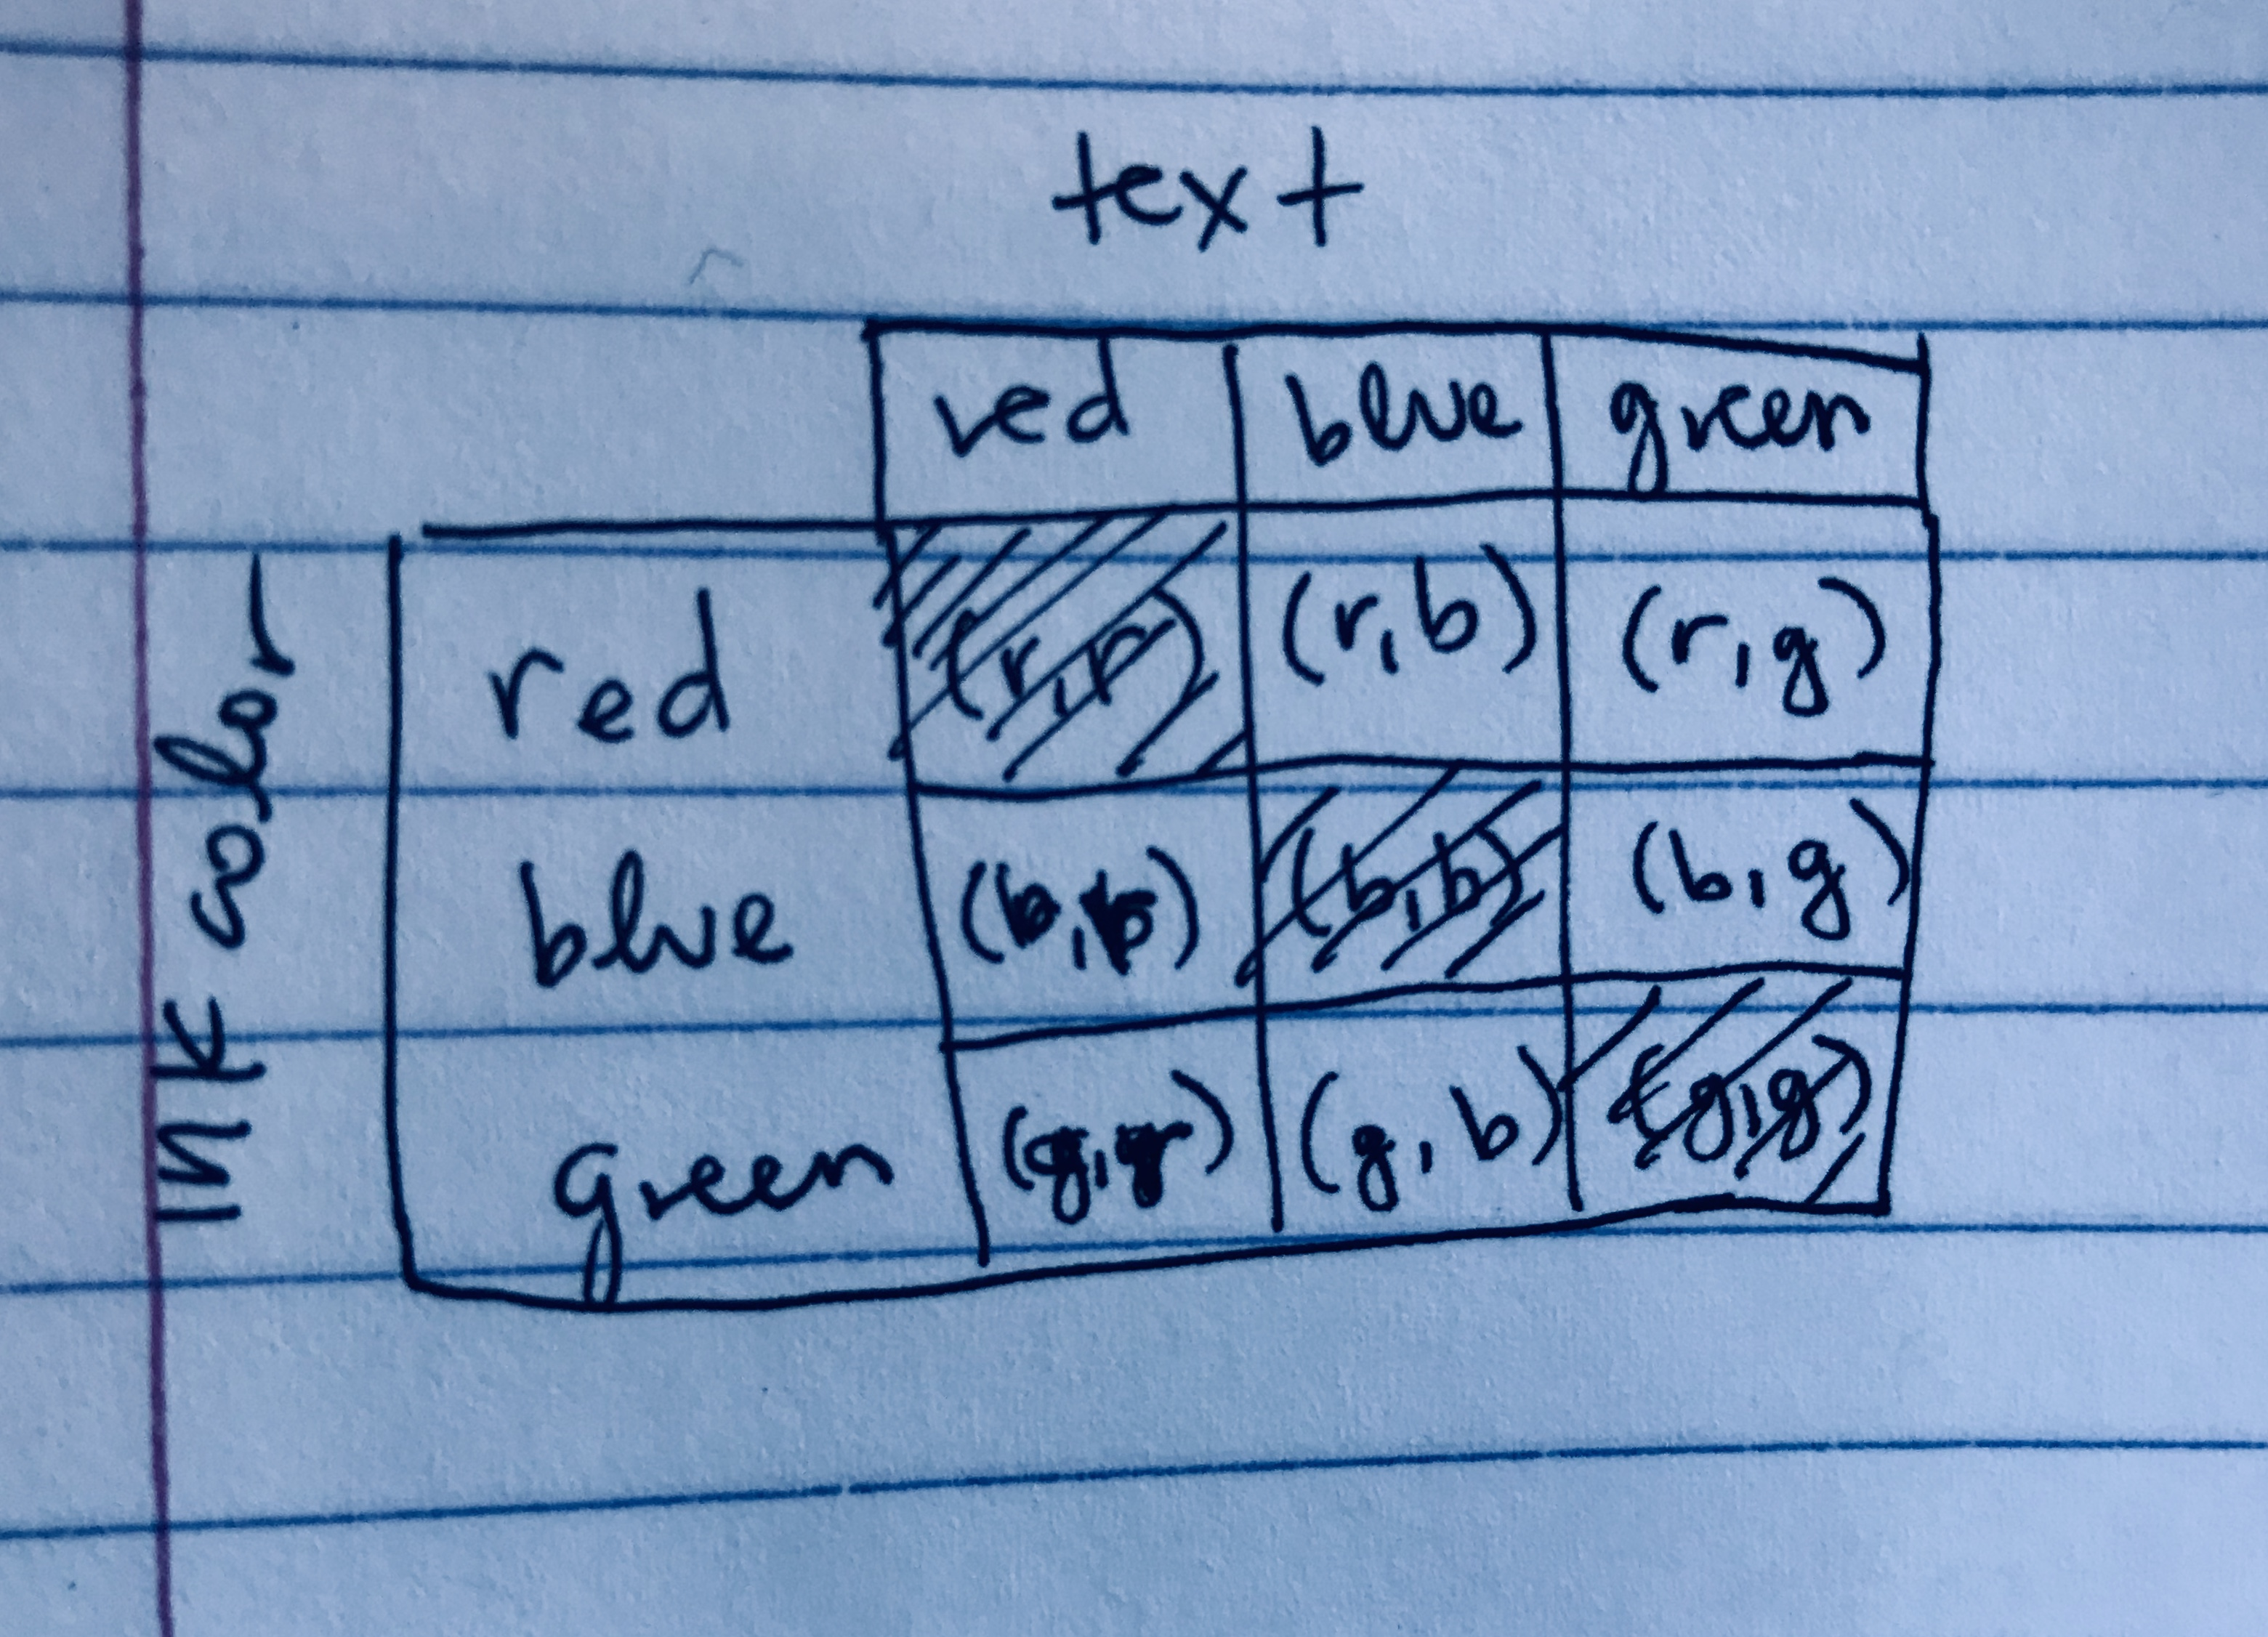
\includegraphics[origin=c,width=10cm]{fig_weighted_crossing}}
%     \caption{Full crossing of a 3 color Stroop experiment. There are more congruent stimuli (along the diagonal) than incongruent stimuli.}%
%     \label{fig:weighted_crossing}%
% \end{figure}
